\chapter{開発したプリンターの精度調査実験}
\label{chp:first}

\section{プリンターの動作検証}
\label{sec:paragraph}
始めに,本研究で開発した氷をマテリアルとした3Dプリンターの動作テストを2つに分けて行った.
1つ目が,プリンターの動作テスト,2つ目が,氷を積層できるかの調査を行った.
この2つの検証をこなうことにより,プリンターの挙動や造形の特徴を知ることができる.

\section{プリンター動作の確認}
\label{sec:paragraph}
一般に販売されているFDM方式の3Dプリンター「 Anycubic i3 Mega S 」を改造して使用している.
ノズルを通常の取り付け位置に設置してしまうと,ノズルの上部が3Dプリンターの上部と接触してしまうため,今回はノズルを左右を繋ぐポールの後ろ側に設置し,そのうえで,ポールから1.5㎝離している.
そのため, Ultimaker Cura で表示されている,印刷が可能な位置と比べ約5cm後ろにずれている.
また,開発した氷をマテリアルとした3Dプリンターの設計上アルミプレートの上でしか造形ができない.
そのため,実際に造形できる範囲は 100mm × 80mm × 250mm であることが分かった.

シリンダーの押し出し機構については,基本的には問題なく作動した.
しかし,3Dプリンターが作動していないタイミングでも,ノズルの先から水が漏れ出してしまうのが問題として発覚した.
また,おそらく水が漏れ出したことに起因して,シリンダー内部の圧力が低下した.この影響により印刷を始めた際にしばらくノズルから水が出ない問題が発生することが分かった.
しかし,現状 Ultimaker Cura の設定により、始めにシリンダーを少し押し出す設定になっている.これにより印刷には影響していないが,対処的な解決策であり,根本的な解決が必要になる.


\section{氷造形の初期実験}
\label{sec:paragraph}
水が綺麗な線が引けて凍るか,積層されるか,開発した氷をマテリアルとした3Dプリンターが実際に氷の造形ができるかをテストした.
線を引く実験では,水と砂糖の割合が1:3のものを使い,印刷速度,押し出し量,ライン幅,の調整を行った.
純粋な水に比べ、砂糖を混ぜた水は凍るまでの速度が遅く,速度を上げすぎると,凍る前に次の層の造形が始まってしまう一方,遅すぎると,ノズルと造形物が凍ってしまい造形ができなくなることが分かった.
押し出し量,ライン幅,については,ノズルの太さ(1mm)を踏まえたうえで,調整しないと,スカスカの造形または,水が飛び出したような造形になってしまう事が分かった.
この時の最適なパラメーターは, ライン幅:3.0mm,印刷速度:50.0mm,押し出し量:300 ということが分かった.
また,アルミプレートの上に直接水を印刷しようとすると途中でプレートから造形物が剥がれてしまい,印刷ができなくなってしまった.
その解決として,アルミプレートの上に濡らしたキッチンペーパーを引くことで解決させた.
キッチンペーパーを造形物とアルミプレートの間に敷くことで、接着面積の増加とキッチンペーパーの繊維に造形物が絡みつくため,外れにくくなった.
また,キッチンペーパーも液体窒素により氷ついているため,造形物をキッチンペーパーから剥がす作業も容易で,キッチンペーパーは複数回使用することが可能だった.
以上の結果とパラメータを基に積層の実験を行った.

\section{氷の積層実験と結果}
\label{sec:paragraph}
氷造形の初期実験で得られた,パラメーターを基に積層に関する実験を行った.
始めに,ライン幅:3.0mm,印刷速度:50.0mm,押し出し量:300,レイヤー高さ:1.0㎜ のパラメータで実験を行った.
この高さでは,押し出し量に対して,高さが足りず、余分な水が外に飛び出し図5.1のような結果が得られた.

\begin{figure}[H]
    \centering
    \includegraphics[width=17truecm]{./fig/sippai.jpg}
    \caption{押し出し量が多すぎた氷の造形物}
  % \url{http://www.this.is.sample.url/} % Web上のデータの場合、参照先URLを明記
    \label{fig:printer2}
  \end{figure}

上記の失敗を基に、パラメーターの調整を行った.
レイヤーの高さを,1.5㎜,2.0㎜,2.5㎜,押し出し量のパラメーターを200,300,に調整して行ったところ,
レイヤー高さを2.0㎜に変更し,押し出し量を200に変更したものが一番綺麗に造形ができたものが図5.2である.
また,水の押し出し量は,フィラメントの押し出し量を調整することで変更できる,
押し出し量の調整は,Arduino IDE を使い,3Dプリンターにアクセスできる.Extrusion multiplier のパラメータで押し出し量を調整することができる.
造形物の大きさは 20mm ×20mm × 9mm の造形物を印刷できた.

  \begin{figure}[H]
    \centering
    \includegraphics[width=17truecm]{./fig/sssa.png}
    \caption{押し出し量を調整して作られた造形物}
  % \url{http://www.this.is.sample.url/} % Web上のデータの場合、参照先URLを明記
    \label{fig:printer2}
  \end{figure}

また,水のみで印刷した際の造形が図5.3である.
水のみの印刷では,水は直ぐに固まってしまう.また,水が一か所に集まろうとして粒が出来上がる.
この粒にさらに水が集まり,しずく状の印刷ムラが多くできてしまう.
このしずく状の印刷ムラがノズルが造形物に干渉し,積層させて印刷をすることができなかった.

\begin{figure}[H]
    \centering
    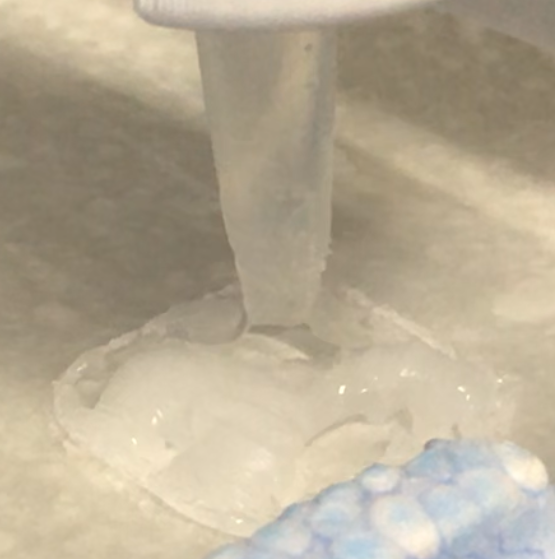
\includegraphics[width=8truecm]{./fig/mizu.png}
    \caption{砂糖を混ぜず水のみでの印刷}
  % \url{http://www.this.is.sample.url/} % Web上のデータの場合、参照先URLを明記
    \label{fig:printer2}
  \end{figure}




